\chapter{Sběr a ukládání dat}
\label{sber-dat}
V~systému RQA se nachází velké množství dat různých formátů. Jedná se například o~videa a fotografie pořízená v průběhu vykonávání testů, datasety obrázků pro trénování algoritmů strojového učení, samotné záznamy o~robotech či zařízeních a mnoho dalších. Dle typu jsou tyto ukládány do~vhodných databází (objektově-relační, dokumentové...). Data, jimiž se práce zaobírá a která popisují chod systému, jsou logy. Logy se vytváří přímo v~kódu programu a ve~větších systémech se často ukládají do specializovaných logovacích systémů. V~případě RQA je tímto Graylog. První dvě sekce této kapitoly se zabývají způsobem zaznamenávání logů na platformě .NET, neboť v~ní je RQA implementováno, a systémem Graylog. Další sekce definují data udávající stav RQA systému a navrhují jejich sběr a formát pro~ukládání do~Graylogu. Následně je ukázán způsob získání dat z~Graylogu a jejich transformace do~vhodného formátu pro~algoritmy strojového učení. Na~závěr je popsána implementace představeného návrhu na platformě .NET.

\section{Zaznamenávání logů v~.NET}
Tato podkapitola vysvětluje principy logování v~.NET. Nejprve je ukázáno, jakým způsobem se logy vytvářejí. Následně je diskutováno, co lze s logy dále dělat. Na závěr jsou představeny možnosti nastavení logování.

\subsection{Vytváření logů v~.NET}
K~vytváření logů slouží objekty implementující \texttt{ILogger} rozhraní obsahující metody k~tomu určené. Pomocí nich lze specifikovat závažnost logu, jeho zprávu, výjimku v~případě chyby nebo argumenty pro~strukturované logování. Typicky se používá generická forma tohoto rozhraní \texttt{ILogger<TCategoryName>}, kde \texttt{TCategoryName} je jméno kategorie, do~které daná instance spadá a na~základě níž lze provádět filtrace nebo upřesňovat nastavení~\cite{logging}.

K~tvorbě instancí \texttt{ILogger} slouží rozhraní \texttt{ILoggerFactory} implementující návrhový vzor továrna. V~rámci tohoto rozhraní lze nastavit, jak se budou konkrétní loggery chovat. Způsob nastavení logování závisí na~tom, zda aplikace využívá tzv. obecného hostitele. Obecný hostitel je objekt, který zapouzdřuje různé zdroje aplikace, jakými jsou například právě logování, konfigurace nebo DI~\cite{generic-host}. Jestliže aplikace tohoto hostitele nepoužívá, nastavení se specifikuje v~metodě \texttt{Create()} rozhraní \texttt{ILoggerFactory}. V~opačném případě nastavení probíhá během konstrukce hostitele v~metodě \texttt{ConfigureLogging()} při~startu aplikace. Toto však nedělá nic jiného, než že \texttt{ILoggerFactory} nastaví za~programátora a vytvářené \texttt{ILogger} instance zpřístupňuje přes DI. Ve~výsledku to programátora od~explicitního používání \texttt{ILoggerFactory} zcela odstíní.

\subsection{Poskytovatelé logování}
\label{poskytovatele-logovani}
Platforma .NET podporuje API, jenž je schopno pracovat s~řadou logovacích poskytovatelů, ať už vestavěných, nebo třetích stran. Logovací poskytovatel slouží k~zobrazování či ukládání logů. Existuje jich velké množství a v~\texttt{ILoggerFactory} se nastavuje, které z~nich se budou používat. Platforma .NET nabízí několik vestavěných poskytovatelů a mnohonásobně více jich existuje od~třetích stran. Nejčastěji se jedná o~open-source projekty sloužící k~posílání logů do~konkrétních logovacích systémů. Oficiální dokumentace Microsoftu~\cite{logging} udává následující vestavěné poskytovatele: 

\begin{itemize}
  \item \emph{Console} --- Logy neukládá, pouze je zobrazuje na standardním výstupu konzole aplikace.
  \item \emph{Debug} --- Slouží k~ladění a typicky logy ukazuje jen ve~vývojovém prostředí.
  \item \emph{EventSource} --- Logy zapisuje do~zdroje událostí v závislosti na~platformě.
  \item \emph{EventLog} --- Lze použít pouze v~prostředí Windows. Logy posílá do~aplikace Windows Event Log.
\end{itemize}

K~běžně používaným externím logovacím poskytovatelům lze zařadit např. GELF nebo Serilog. Tyto zajišťují strukturované logování do vlastních logovacích systémů (Graylog a Serilog). Strukturované logování umožňuje přidávat logům dodatečné argumenty, které se pak v~logovacím systému převedou na~zvláštní pole jako na obrázku~\ref{structured-log-img}.

\begin{figure}[hbt]
	\centering
	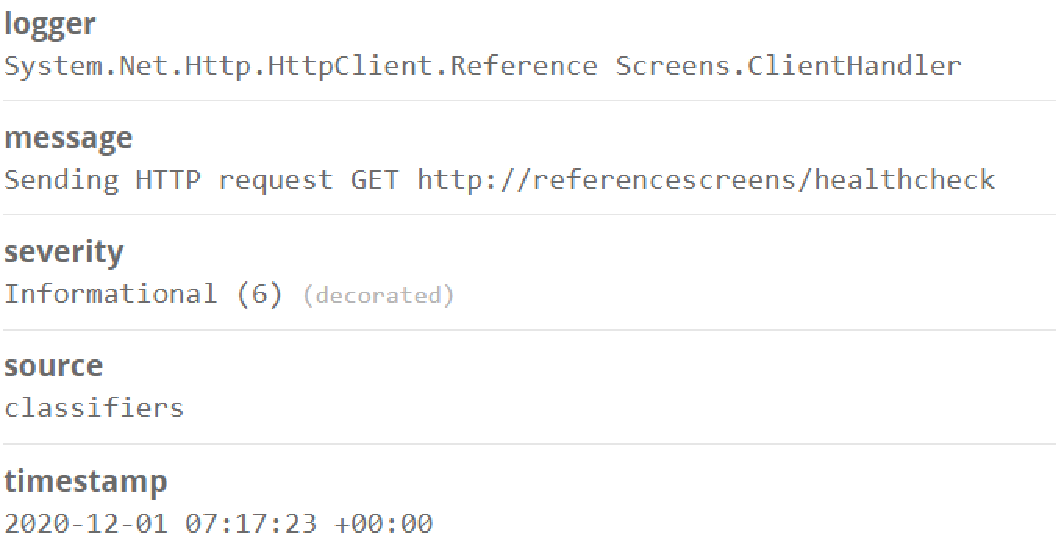
\includegraphics[width=0.85\textwidth]{obrazky/structured-log.pdf}
	\caption{Ukázka části strukturovaného logu v~systému Graylog}
	\label{structured-log-img}
\end{figure}

Pro doplňování logů o~dodatečné informace, ve~strukturovaném nebo nestrukturovaném formátu, lze využít logovací rámce. \texttt{ILogger} rozhraní obsahuje metodu \texttt{BeginScope()}, do~jejíchž parametrů lze danou informaci předat v~různém formátu v~závislosti na přetížení metody~\cite{logging, ilogger-beginscope}. Tato pak vytvoří jednorázový rámec, v~němž se ke~všem logům přidá specifikovaná informace bez nutnosti ji opakovaně udávat.

\subsection{Konfigurace logování}
Již bylo řečeno, že poskytovatelé logování se nastavují v~\texttt{ILoggerFactory}. Toto rozhraní umožňuje vytvořit i filtrovací pravidla, díky nimž lze logy zaznamenávat pouze od~určité úrovně závažnosti či jen z~vybraných kategorií~\cite{logging}. Mimo nastavení \texttt{ILoggerFactory}, které platí jen pro danou instanci~\cite{logging}, je možné logování konfigurovat i globálně. K~tomu slouží sekce \texttt{Logging} v~souboru \emph{appsettings.json}, v~němž bývají všechna potřebná nastavení .NET aplikací. Zde se nastavují parametry jednotlivých poskytovatelů, jako například adresa serveru s~logovacím systémem, port, protokol atd. Dále tu lze specifikovat výchozí úrovně závažnosti logů či filtry, ať už pro dané poskytovatele, nebo jen jejich kategorie.

\section{Graylog}
\label{graylog}
RQA používá pro~ukládání logů open-source logovací systém Graylog. Do něj se zapisuje již zmíněným GELF (Graylog Extended Log Format) poskytovatelem a už z~významu zkratky je patrné, že používá speciální formát logů pro~Graylog. V~zásadě se tento formát snaží zbavit nedostatků standardního logovacího formátu syslog, jako například omezená velikost, beztypovost nebo nemožnost komprese, a především je strukturovaný~\cite{gelf}. Pro~použití poskytovatele v~prostředí .NET je potřeba nainstalovat NuGet balík \emph{Gelf.Extensions.Logging}.

V~samotném systému Graylog lze s~logy pracovat různými způsoby. Především slouží k~vyhledání chybových zpráv v~případě, že je v~cílové aplikaci těžko dohledatelná chyba. Nabízí řadu widgetů pro~vizualizaci a práci s~logy. Umí logy předfiltrovat do~tzv. streamů, což je pouze název Graylogu pro~kategorii. Toto potom zlepšuje celkovou přehlednost nebo i rychlost vyhledávání. Významnou vlastností je také schopnost zasílat upozornění v~případě, že dojde k~nějaké události. Tato je definovaná určitou podmínkou, kterou musí příchozí log splňovat.

\section{Metriky vypovídající o stavu RQA systému}
Existuje řada metrik, jichž se používá při~monitorování systémů a aplikací. Těmito mohou být fyzické prostředky (vytížení procesoru, využití paměti RAM...), síťové parametry (propustnost, latence, ztráta paketů...) nebo aplikačně specifické metriky (návštěvnost webu...). Jelikož je žádoucí, aby RQA pracovalo efektivně a s minimálním počtem chyb, za metriky byly zvoleny délky zpracování požadavků mikroslužbami a chybovost. Následující sekce tuto volbu dále vysvětlují.

\subsection{Délka zpracování požadavku službou}
\label{delka-zpracovani-pozadavku}
Vzhledem k~architektuře mikroslužeb systém generuje nemalý síťový provoz. Většina akcí je prováděna voláním služeb, a~proto je důležité, aby délka zpracování jednotlivých požadavků byla relativně stabilní. Není tu však řeč o~času ztráveném čekáním na~odpověď klientem. Tento čas v~sobě zahrnuje i latenci, která je ovlivněna rychlostí a stabilitou sítě, k~níž je uživatel připojen. Nepřiměřená délka požadavku by tedy nemusela být zapříčiněna vadou systému, pouze pomalou lokální sítí uživatele, a anomálie by se detekovala chybně. Metrikou je míněna doba, která uplyne od~přijetí požadavku službou po~odeslání její odpovědi. Naměřený čas je tedy skutečně pouze ten, za~nějž je systém zodpovědný. Argumentovat lze případem, kdy služba volá ještě jinou službu. Latence a ostatní síťové prvky tohoto volání pak jsou v tomto čase zahrnuty. Služby však běží stále na~stejné síti, navzájem jsou pořád stejně vzdálené, a~proto tato latence bude víceméně stabilní. Rozhodně by problém zde nebyl zapříčiněn externím elementem. Případná detekce anomálie by tedy byla v~pořádku.

\subsection{Chybovost}
Chybovost lze považovat za~zřejmě nejzákladnější metriku určující stav prakticky jakéhokoliv systému i mimo obor informačních technologií. Systém by měl vykazovat minimální množství chyb, a~proto má rozhodně cenu jejich nestandardní množství detekovat. Zaznamenávat by se měly všechny možné druhy chyb během požadavku. Mezi ty patří například fatální neošetřené chyby způsobující konec provádění požadavku, ošetřené, jež provádění rozumně ukončí, nebo takové, z nichž se služba dokáže vzpamatovat.

\subsection{Nevhodné metriky}
\label{nevhodne-metriky}
Tato sekce slouží k~vysvětlení, proč některé běžně používané metriky v~oblasti monitorování aplikací a systémů nejsou použitelné pro~zadaný problém.

\subsubsection{Latence}
Latence již byla probírána v~sekci~\ref{delka-zpracovani-pozadavku}, kde se nastínilo, že je závislá na~lokální síti uživatele. Z~toho důvodu moc přesně nevypovídá o~stavu systému samotného. Dalším problémem je způsob měření. Buď by se muselo provádět externím nástrojem, nebo by každé jedno volání v~celém systému muselo být obaleno časovačem, jenž by ho měřil. První možnost by snížila soběstačnost RQA a druhá nepřipadá v úvahu, neboť by vyžadovala extrémní zásahy do~kódu a navíc se nejedná o~dobrou praktiku.

\subsubsection{Využití šířky pásma}
Využití šířky pásma (brandwidth usage) není vhodnou metrikou, neboť udává informaci o~stavu sítě, v~níž se systém nachází, nikoliv o~systému jako takovém. I~kdyby se filtroval síťový provoz generovaný jen od~RQA, je jednak nutno ho měřit externě a jednak je získaná informace zcela zbytečná. Síťová aktivita RQA totiž závisí na~tom, jestli a kolik zrovna běží testů nebo kolik uživatelů systém aktuálně používá. Tato informace je tedy variabilní a žádné systémové anomálie v~ní proto není možné hledat.

\subsubsection{Využití procesoru a operační paměti RAM}
Tyto metriky nelze měřit, neboť jsou požadavky na~služby vytvářeny asynchronně. Tím se ve~fondu vláken (\texttt{ThreadPool}) naplánuje vykonání práce a~pak již téměř nelze určit, které vlákno patří kterému požadavku~\cite{threadpool}. O~to více pak věci komplikuje kontejnerizace prvků systému a jejich nasazení v~Kubernetes. Tato platforma se navíc o~tento typ monitorování stará sama.

\section{Získání a uložení hodnot metrik}
V~této podkapitole je popsáno měření potřebných údajů a jejich zaznamenávání do~systému Graylog. Pro~tento účel se využívá koncept zvaný middleware, jenž je vysvětlen v~nadcházející sekci. Dále se rozebírá přesný způsob získání a logování informací o~požadavcích služeb a chybách. Na~závěr je ukázána organizace vytvořených logů v~Graylogu.

\subsection{Middleware v~ASP.NET}
Middleware je software, jenž se provádí před a po~zpracování každého požadavku, jako je vyobrazeno na~obrázku~\ref{middleware-img}. Požadavek či odpověď je tedy možné modifikovat. Obecně ho však lze použít pro~spuštění libovolného kódu. Metodou \texttt{Next()} se middleware opustí a pokračuje se ve~vykonávání požadavku.

\begin{figure}[hbt]
	\centering
	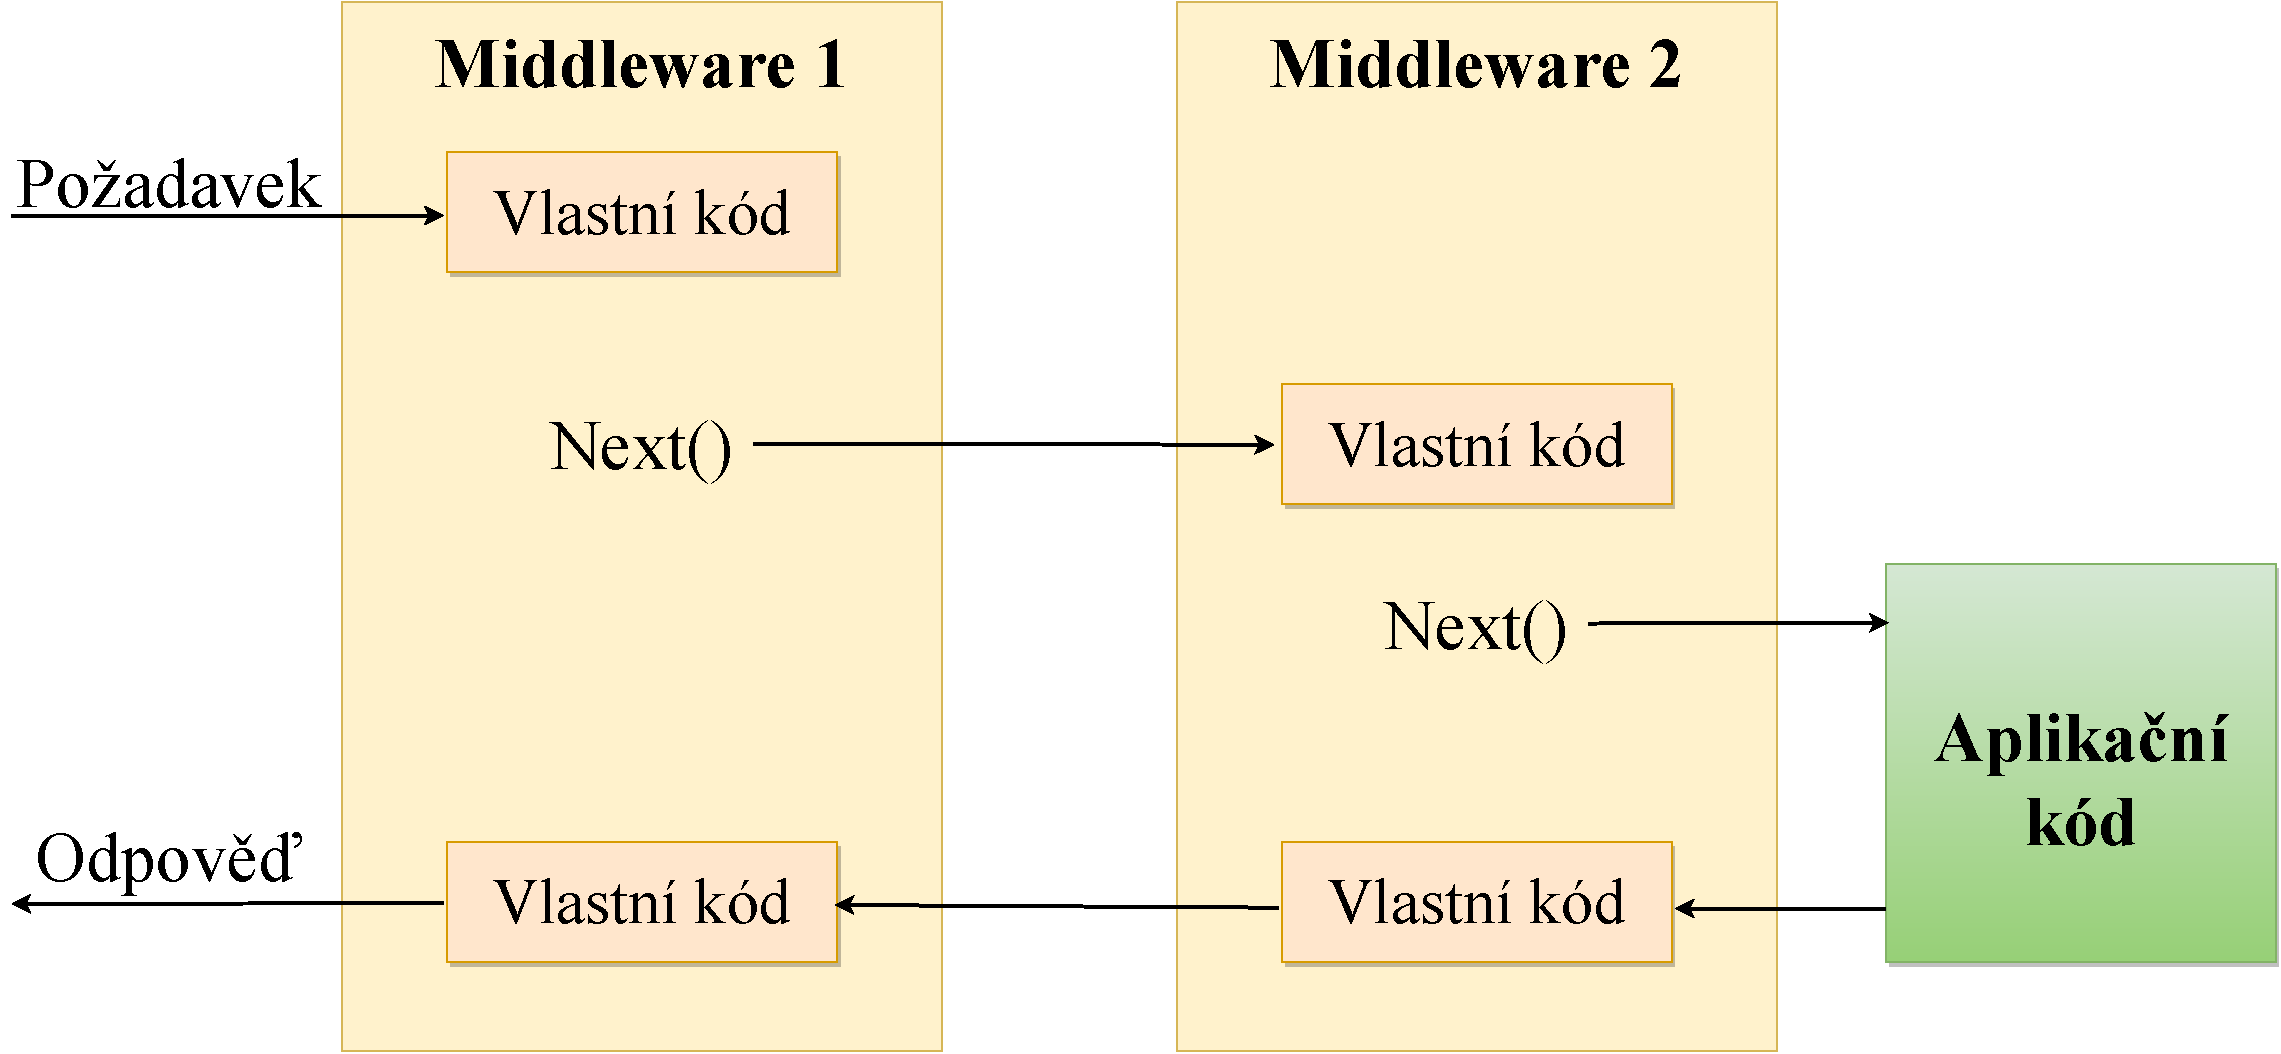
\includegraphics[width=0.9\textwidth]{obrazky/middleware.pdf}
	\caption{Princip provádění middlewaru v~ASP.NET}
	\label{middleware-img}
\end{figure}

K~plnému pochopení middlewaru je záhodno vysvětlit, jak na~platformě ASP.NET funguje zpracování webových požadavků. Klientská aplikace zašle požadavek na webový server, kde se vytvoří kanál zpracování požadavku dle konfigurace definované třídou \texttt{Startup}, v~rámci níž se mimo jiné právě middlewary registrují~\cite{middleware}. Zpracování se následně přesune do~jednotlivých middlewarů v~pořadí, v~jakém byly registrovány. Až poté teprve přijde na~řadu aplikační kód. Stejnou cestou se pak putuje zpět k~webovému serveru, který odešle odpověď. 

\subsection{Zaznamenání údajů o požadavcích na služby}
\label{zaznamenani-udaju-o-pozadavcich-na-sluzby}
Pro~vytváření logů o~délkách zpracování požadavků slouží middleware, jenž se jednotlivým mikroslužbám pouze zaregistruje. Měření probíhá tak, že se v~první fázi middlewaru spustí stopky a na~zpáteční cestě se zastaví, načež dojde k~zalogování informace.

Mimo samotnou délku požadavku je však zapotřebí mít i jiné údaje. Těmi jsou časové razítko a cíl požadavku, aby se vědělo, čeho délka se měří. Čas zaznamenání logu doplňuje ASP.NET automaticky všem logům, a~tak tento údaj není nutné řešit. Jedná se prakticky o~konec vykonávání požadavku a jeho začátek lze snadno dopočítat odečtením jeho délky. Původ logu je již taktéž znám. V~konfiguraci logování v~souboru \emph{appsettings.json} každé mikroslužby se zdroj definuje jako její název. Toto však samo o~sobě nestačí. Různé požadavky v~rámci stejné služby stále trvají odlišnou dobu, proto je třeba zaznamenat přesný cíl požadavku, kterým je dvojice kontrolér-akce. Tuto informaci pak lze vyčíst z~kontextu volání \cite{route-data}.

Logy, z~nichž se detekují anomálie v~délkách zpracování požadavků, tedy obsahují následující argumenty: časové razítko (timestamp), délka požadavku (duration), jméno služby (source), jméno kontroléru a akce (requestHandler).

\subsection{Zaznamenání údajů o chybách}
\label{zaznamenani-udaju-o-chybach}
Tato část práce řeší ten problém RQA, že aktuálně není zaznamenávání chyb v~systému jednotné. Chyby ve~službách většinou nejsou ošetřeny, neboť UI systému se o~nich nějak musí dozvědět, aby informovalo uživatele o~nezdařené akci. Z~toho důvodu nevadí nechat chybu propagovat jako klasickou interní chybu~500. Nicméně, takhle chyby kontroluje a loguje právě UI, čímž se z~pohledu logování stává zdrojem dané chyby. Zdroj je však pro~účely detekce anomálií důležitý, a~tak se logování musí dít již na~straně služby.

Implementačně nejčistším řešením je rozhraní \texttt{IExceptionFilter}. To umožňuje provádět akce nad~neošetřenými výjimkami. Dojde-li k~nějaké, provádění programu se přesune do~metody \texttt{OnException()}, v~níž lze log vytvořit. Není tedy potřeba upravovat kód v~celém systému a zanášet ho \texttt{try-catch} bloky. Problém tohoto řešení však spočívá v~tom, že pokud se vytvoří chybový log a výjimka se přepošle, aby se vypropagovala ven ze~služby, tok programu již neprojde zpětně žádným middlewarem. Nedojde tedy k~zaznamenání volání služby, jež probíhá právě v~tomto místě. Jednoduchou alternativou rozhraní \texttt{IExceptionFilter} je použití middlewaru s~metodu \texttt{Next()} vloženou do~\texttt{try} bloku. Tímto způsobem lze před přeposláním výjimky zaznamenat kromě chyby i konec požadavku. Je proto výhodné toto provádět v~middlewaru měřícím délku zpracování požadavku, neboť ten jediný má právě onu délku potřebnou pro~zaznamenání konce požadavku.

Občas je ale žádoucí chybu ošetřit a log vytvořit ručně. To by znamenalo, že by se u~každého logu musel specifikovat jeho zdroj, jímž je stejně jako u~délky zpracování požadavků dvojice kontrolér-akce. Zde přichází na~řadu metoda \texttt{BeginScope()} rozhraní \texttt{ILogger}, jež byla představena na~konci sekce~\ref{poskytovatele-logovani}. Jak to tedy provést jednoduše? Vytvoří se middleware, který pouze vytvoří logovací rámec, jenž bude logům přidávat informaci o~kontroléru a jeho akci. Vzhledem k~povaze middlewaru je tento rámec platný pro~celé volání služby. Zdroj se tedy automaticky doplní každému logu. Podmínkou tohoto přístupu je však registrace nativního routing middlewaru, tedy zavolání ASP.NET metody \texttt{UseRouting()}, před~registrací výše zmíněného. Pro~zjištění cíle požadavku je totiž zapotřebí mít již routing zprovozněn. Dále pokud se zaregistruje middleware vytvářející logovací rámec dříve než middleware, který měří délku zpracování požadavků a zachytává chyby, může se z~druhého taktéž odstranit explicitní přidávání argumentu o~kontroléru a akci. Tento předpoklad lze zajistit zpřístupněním metody, jež je zaregistruje ve~správném pořadí.

Pole chybových logů, která jsou potřebná a budou zajištěna, jsou následující: časové razítko (timestamp), jméno služby (source) a jméno kontroléru a akce (requestHandler). Chybová hláška či výjimka pro~detekci anomálií nejsou podstatné.

\subsection{Zpracování záznamů v systému Graylog}
V~podkapitole~\ref{graylog} byl vysvětlen pojem stream systému Graylog. Do~dvou takových streamů jsou logy kategorizovány. Dosahuje se tím vyšší přehlednosti, rychlosti při filtraci a tedy i stahování dat. První stream je pro~logy s~délkami zpracování požadavků. Takový log se pozná podle toho, že obsahuje všechna pole zmíněná v~sekci~\ref{zaznamenani-udaju-o-pozadavcich-na-sluzby}. Ve~druhém streamu se uchovávají chybové logy. Zda se jedná o~chybový log, se zjistí z~implicitního pole úrovně logu (\texttt{level}). Toto pole obsahuje každý log a pro~chybu je jeho hodnota~3. Z~nich se však budou brát v~potaz jen ty s~platným polem \texttt{requestHandler} kvůli webovému UI. Tam totiž mohou vznikat chyby zapříčiněné uživatelem nebo může dojít k~opětovnému zalogování chyby služby, která již byla danou službou zaznamenána, tentokrát však z~pohledu klienta, že nedostal platná data. Existence pole \texttt{requestHandler} zaručí, že k~chybě došlo v~logice webu, jeho kontroléru, a ne někde jinde.

\section{Tvorba kolekce dat ze zaznamenaných logů}
V~této fázi návrhu jsou již všechna potřebná data na~jednom místě, a sice v~Graylogu. Posledním krokem je transformovat logy na~data použitelná pro~nějaký algoritmus. Brát je přímo z~Graylogu není vhodné ze dvou důvodů. Logů ke~zpracování existují miliony, a~proto by každá detekce kvůli jejich stažení zabrala extrémně dlouho. Dále pak logy obsahují mnoho polí, která nejsou vůbec potřeba. Zjednodušení dat tedy značně sníží nároky na~paměť. V~následujících sekcích je navržen způsob stažení logů z~Graylogu, jejich transformace do~vhodného formátu a uložení na~straně aplikace detekce anomálií.

\subsection{Stažení dat pomocí Graylog REST API}
Získat data z~Graylogu bohužel není tak snadné, jak by se mohlo na~první pohled zdát. K~vyhledávání totiž využívá software Elasticsearch, jenž je limitován zobrazením pouze~10~000 položek najednou z~důvodu paměťové náročnosti~\cite{graylog-limit}. Proto nelze více než tento limit nejen zobrazit přímo v~Graylogu, ale ani stáhnout pomocí Graylog REST API, jež webové rozhraní stejně používá~\cite{graylog-api}. Limit lze sice navýšit, nicméně potom je vyžadováno výrazně více paměti a procesoru, což může zapříčinit snížení výkonnosti nebo i vznik chyb~\cite{elastic-limit}. Tento limit tedy není doporučeno měnit, a~tak nezbývá než logy stahovat po~dávkách.

Graylog REST API nabízí dvě formy vyhledávání, relativní a absolutní. U~relativního se čas specifikuje v~minutách, do~kterého se chtějí vyhledat logy od~aktuálního času. Za~normálních okolností by toto bylo preferované, avšak tím, že je nutno stahovat po~dávkách, by se s~každou dávkou posunulo časové okno. Dále by mohly nastat nepřesnosti spjaté s~latencí. Výhodnější je použít absolutní vyhledávání, které je od~pevného začátku do~pevného konce.

Chtějí-li se tedy stáhnout logy z~intervalu T\textsubscript{1} až T\textsubscript{2}, typicky od~nějakého bodu v~minulosti do~aktuálního času, vyšle se požadavek na~stažení dat z~tohoto intervalu. Stáhne-li se méně než limitních 10~000 logů, bylo staženo vše z~tohoto intervalu. Pokud však odpověď obsahuje právě tento limitní počet, nestáhlo se vše, čas T\textsubscript{1} se nastaví na~hodnotu časového razítka posledního staženého logu a vyšle se další požadavek na~stažení. Takto se stahuje po~dávkách o~10~000 záznamech, dokud se nestáhne dávka s~nižším počtem signalizující konec stahování.

\subsection{Zpracování a uložení dat}
\label{zpracovani-a-ulozeni-dat}
Vzhledem k~obrovskému množství logů, jehož stahování trvá dlouho a zdržovalo by detekci, se tyto ukládají na~straně aplikace provádějící detekci anomálií v~podobě CSV souborů. Každý typ požadavku jednotlivých služeb má svůj vlastní a to jak pro~již zanalyzovaná referenční data, tak pro~nová a doposud nezpracovaná data. Aplikace si tak udržuje všechna potřebná data a při~požadavku na~provedení detekce již nic nestahuje, pouze provede analýzu nad~doposud nezpracovanými daty. Obrázek~\ref{log-download-infrastructure-img} zobrazuje putování dat.

\begin{figure}[hbt]
	\centering
	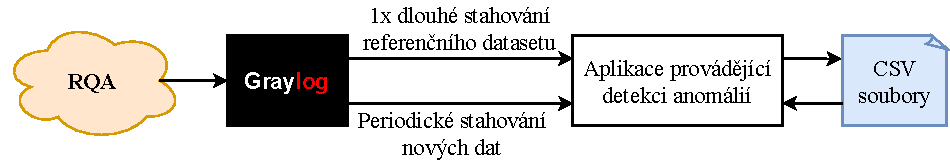
\includegraphics[width=1\textwidth]{obrazky/log-download-infrastructure.pdf}
	\caption{Komponenty podílející se na sběru dat}
	\label{log-download-infrastructure-img}
\end{figure}

Miliony referenčních logů se tedy stáhnou jen jednou a dataset se vyčistí dle postupu v~sekci~\ref{cisteni-kolekce-dat}. Nové logy se pak stahují už jen pro~krátký interval od~posledního staženého logu po~aktuální čas. Délka intervalu závisí na~frekvenci průběžného stahování. Novými logy se pak CSV soubory upravují. Úprava probíhá následovně. Nechť v~CSV souborech existují logy z~referenčního intervalu, například za~poslední týden, a nová data se stahují s~určitou periodou, třeba pět minut. Průběžně se tedy stahují logy za~cca předešlých pět minut podle posledního staženého logu a přidávají se do~souborů s~doposud nezpracovanými daty. S~požadavkem na~detekci anomálií, který je nezávislý na samotném stahování, se tyto zpracují, přidají do referenčního datasetu a naopak referenční logy starší než týden se smažou pro~zachování týdenního referenčního intervalu. Tímto způsobem se budou data neustále aktualizovat.

Před~zápisem do~CSV souborů je ještě potřeba stažené logy upravit do~vhodného formátu. Toho se docílí tím, že se pro~logy požadavků a chyb vytvoří samostatné třídy s~atributy pro~vybraná pole logů (viz~\ref{zaznamenani-udaju-o-pozadavcich-na-sluzby} a~\ref{zaznamenani-udaju-o-chybach}). Do~nich se logy z~formátu JSON deserializují a rovnou tím dojde ke zbavení se nepotřebných dat.

Princip samotného algoritmu pro~dávkové stahování a ukládání logů je popsán vývojovým diagramem v~příloze~\ref{priloha-C}. V~zásadě se nejdříve zvolí délka intervalu, z~něhož jsou logy požadovány od~aktuálního času. Poté se stáhnou všechny chybové logy. Těch nejsou miliony, takže není problém je mít prozatímně uložené v~paměti. Dále jsou stahovány dávky logů s~požadavky. Pro~jednotlivé požadavky se počítají chyby, které v~nich vznikly, a údaje se zapisují do~CSV souborů. Vzhledem k~tomu, že soubory jsou již rozděleny dle služeb a typů požadavků, zapsány jsou už jen časové razítko, délka požadavku a počet chyb jako ukazuje obrázek~\ref{csv-format-img}. Konec stahování indikuje to, že poslední dávka již není plná. V~případě stahování referenčních dat, které může trvat i hodiny, je třeba ještě zpětně stáhnout logy vzniklé během stahování. Jakmile budou data dostatečně aktuální, může se spustit samotná detekce.

\begin{figure}[hbt]
	\centering
	\begin{boxedverbatim}
Timestamp,Duration,Errors
18/01/2021 09:55:42.311 AM,37.1783,0
	\end{boxedverbatim}
	\caption{Výsledný formát dat v~CSV souboru}
	\label{csv-format-img}
\end{figure}


\section{Implementace sběru a přípravy dat}
\label{implementace-sberu-dat}
Sběr dat z~RQA do~Graylogu i stahování dat z~Graylogu je implementováno samostatnými projekty formou knihoven popsaných níže. Detekční aplikací zmíněnou v~předchozí sekci proto může být prakticky cokoliv. Konkrétní program není v~rámci řešení implementován. Pro~úplnost je však vhodné uvést všechny projekty řešení:

\begin{itemize}
  \item \emph{AnomalyDetection} --- Jedná se o~jedinou spustitelnou aplikaci řešení v~podobě webového API. Toto obsahuje pouze pár endpointů pro~stahování logů z~Graylogu a mazání stažených logů na~straně tohoto API. Ke~svému chodu využívá knihovnu \emph{AnomalyDetection.Data}, o~které bude řeč níže, žádnou vlastní logiku neimplementuje. API je snadno rozšiřitelné i pro~ovládání samotné detekce anomálií.
  \item \emph{AnomalyDetection.Application} --- Projekt implementuje detekci anomálií a je popsán v~kapitole \ref{implementace-detekce-anomalii}.
  \item \emph{AnomalyDetection.Client} --- Jednoduchý malý projekt, který slouží ke~generování klienta pro~výše zmíněné webové API pomocí nástroje NSwag.
  \item \emph{AnomalyDetection.Data} --- Obsahuje implementaci stahování dat z~Graylogu, jejich úpravy, transformace do~formátu CSV a uložení na~straně aplikace využívající tuto knihovnu.
  \item \emph{AnomalyDetection.Metrics} --- Implementuje middlewary sbírající potřebná data.
\end{itemize}

Úkolem projektu \emph{AnomalyDetection.Data} je připravit data pro~detekci anomálií. Největší podíl na~tom mají třídy \texttt{CsvHandler} a \texttt{GraylogProvider}. \texttt{CsvHandler} se stará o~veškerou práci s~CSV soubory, k čemuž využívá knihovnu \emph{CsvHelper}. Třída \texttt{GraylogProvider} pak implementuje algoritmus z~přílohy \ref{priloha-C}. Její velkou částí je vytváření dotazového url na~Graylog REST API. To vrací logy ve formátu JSON, které třída deserializuje, roztřídí podle služeb a typů požadavků a uloží pomocí \texttt{CsvHandler} do~CSV souborů tak, jak je popsáno v~sekci~\ref{zpracovani-a-ulozeni-dat}. Při~práci s~touto třídou je důležité mít na~paměti, že Graylog pracuje v~UTC čase, a~proto jsou místy nutné převody. Vlastnost \texttt{UtcHoursDiff} poskytuje rozdíl mezi lokálním a UTC časem.

V~projektu \emph{AnomalyDetection.Metrics} lze nalézt dva middlewary reflektující návrh popsaný v~sekcích~\ref{zaznamenani-udaju-o-pozadavcich-na-sluzby} a~\ref{zaznamenani-udaju-o-chybach}. Middleware \texttt{RequestDestinationMiddleware} si z~kontextu volání vytáhne název kontroléru a akce, na~něž je požadavek směřován, a vytvoří globální logovací rámec přidávající logům informaci o~cíli požadavku. Každý log vytvořený během požadavku tak bude obsahovat dodatečné pole \texttt{requestHandler} s~hodnotou \uv{\{kontrolér\}-\{akce\}}. Druhým middlewarem je \texttt{RequestDurationMiddleware}, jenž před zahájením požadavku pouze spustí stopky a na~jeho konci vytvoří log informující o~délce požadavku. Zároveň zachytává a zaznamenává všechny neošetřené chyby, neboť dělo-li by se to jinde, chyba by se propagovala tam. Vykonávání požadavku by se již nikdy nevrátilo do~tohoto middlewaru, a nezaznamenala by se proto délka onoho chybového požadavku. Projekt dále zprostředkovává metodu \texttt{UseAnomalyDetection()} pro~registraci middlewarů do~kanálu zpracování požadavku. Zahrnutí nějaké služby do~detekce anomálií je tedy natolik jednoduché, že tuto metodu pouze stačí zavolat v~metodě \texttt{Configure()} třídy \texttt{Startup} dané služby.